\section{Experiments}\label{sec:experiments}
We design our experiments to understand how well our algorithm behaves on real-world datasets and how
it compares to the state-of-the-art approaches. As pointed out in Section~\ref{sec:intro}, we are not
aware of a scalable approach for solving the {\it multi-dimensional} balanced partitioning. Hence, 
we present a quantitative comparison of \algnameshort with related techniques for {\it one-dimensional} variant
of the problem. The experiments for multi-dimensional variant are discussed in Section ~\ref{sec:multi-exp}.

For our experiments, we use three publicly available social networks\footnote{The data is available at \url{https://snap.stanford.edu/data}} 
and several large subgraphs of the Facebook friendship graph. We utilize the public graphs for which the results of the state-of-the-art minimum-cut partitioning are known. The private datasets serve to demonstrate scalability of our approach and its performance on real-world data. Our dataset is as follows.

\begin{compactitem}
    \item \texttt{LiveJournal} is an undirected version of the public social graph (snapshot from 2006) containing $4.8$ million vertices and $42.9$ million edges~\cite{UB13}.

    \item \texttt{Twitter} is a public graph of tweets, with about $41$ million vertices (twitter accounts) and $1.2$ billion 
    edges (denoting followership)~\cite{Kwak10}.

    \item \texttt{Friendster} is another public social network whose minimum-cut partitioning is 
    available~\cite{ABM16}; it contains $65$ million edges and $1.8$ billion edges.

  \item \texttt{FB-X} are subgraphs of the Facebook friendship graph, where $X$ indicates the (approximate) number of edges; the data was anonymized before processing.
\end{compactitem}

\subsection{One-dimensional partitioning}
We evaluate our algorithm, denoted by \algnameshort and described in Section~\ref{}, with existing scalable approaches for graph partitioning. Recall that our primary goal is to design and implement a scalable algorithm that can run for very large graphs in distributed setting.
The most relevant works are the label propagation-based approaches by Ugander and Backstrom~\cite{UB13} and by Martella at al.~\cite{MLLS17}, balanced partitioning via linear embedding by Aydin et al.~\cite{ABM16}, a streaming technique, called Fennel, suggested by Tsourakakis et al.~\cite{TGRV14}, and a distributed local search-based algorithm, SocialHash, by Kabiljo at al.~\cite{SH16,KKPPSAP17}. We also include results computed by the classical library for graph partitioning, METIS~\cite{KK95}.

\begin{table}[!h]
	\centering
	\begin{tabular}{lrrrrrr}\toprule
		\multicolumn{1}{c}{Graph} & \multicolumn{1}{c}{\algnameshort} %
		& \multicolumn{1}{c}{SocialHash} & \multicolumn{1}{c}{LinEm} & \multicolumn{1}{c}{Spinner} & \multicolumn{1}{c}{Fennel} & \multicolumn{1}{c}{METIS} \\
		\midrule
		\texttt{Twitter}
		& $7.3\%$ & $8.33\%$ & $7.43\%$ & $15\%$ & $\boldsymbol{6.8\%}$ & $11.98\%$ \\
		& $\eps=0.02$ & $\eps=0.01$ & $\eps=0.03$ & $\eps=0.05$ & $\eps=0.1$ &$\eps=0.03$ \\
		\midrule
		\texttt{Friendster}
		& $3.73\%$ & $\boldsymbol{3.54\%}$ & $11.9\%$ &  &  &  \\
		& $\eps=0.03$ & $\eps=0.01$ & $\eps=0.03$ &  &  &  \\
		\bottomrule
	\end{tabular}
	\vspace{0.1cm}
	\caption{bla.}
	\label{table:quality}
\end{table}

Table~\ref{table:quality} compares the percentage of cut edges produced by various algorithms. Although the new 
algorithm, \algnameshort, does not always provide the lowest edge cut, it generally produces high quality partitions. 
We believe that a careful engineering and tuning of our approach might result in lower edge cuts.
For the Facebook graphs, described in Table~\ref{table:qualityFB}, we computed solutions using partitioners
that provide open source implementations. Observe that our algorithm
finds best solutions for all but one instance, making it an attractive option for the dataset. 

\begin{table}[ht]
	\begin{minipage}[b]{0.5\linewidth}
		\centering
		\begin{tabular}{lrr}
			\toprule
			\multicolumn{1}{c}{Graph} & \multicolumn{1}{c}{\algnameshort} %
			& \multicolumn{1}{c}{SocialHash} \\
			\midrule
			\texttt{FB-2.5B}
			& $\boldsymbol{5.11\%}$ & $8.75\%$ \\
			\texttt{FB-5.5B}
			& $\boldsymbol{4.99\%}$  & $11.75\%$ \\
			\texttt{FB-80B}
			& $\boldsymbol{5.21\%}$  & $12.04\%$ \\
			\texttt{FB-400B}
			& $6.88\%$  & $\boldsymbol{5.82\%}$ \\
			\texttt{FB-800B}
			& $\boldsymbol{5.52\%}$  & $5.58\%$ \\
			\bottomrule
		\end{tabular}
		\vspace{0.3cm}
		\caption{bla.}
		\label{table:qualityFB}
	\end{minipage}\hfill
	\begin{minipage}[b]{0.48\linewidth}
		\centering
		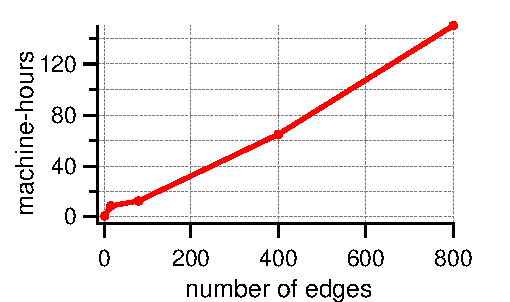
\includegraphics[width=0.9\textwidth]{pics/mt}
		\vspace{0.05cm}
		\captionof{figure}{Scalability bla.}
		\label{fig:mh}
	\end{minipage}
\end{table}

In order to compute results for the largest instances with billions of edges, we implemented \algnameshort in a
vertex-centric programming model and ran experiments in a distributed graph processing system, Giraph\footnote{\url{http://giraph.apache.org}}; similar
implementations exist for Spinner~\cite{MLLS17} and SocialHash~\cite{KKPPSAP17}.
In Giraph, a computation is split into a number of supersteps that end with a synchronization barrier.
Every superstep executes a user-defined function based on local vertex data, and sends and receives
messages from adjacent vertices. Algorithm~\ref{alg:mdgp-rpgd} can naturally be implemented in the
vertex-centric model, as computing gradients requires information about its neighbors.
As a measure of scalability of our implementation, we report in Figure~\ref{fig:mh} the running time in machine-hours
on a cluster of a few tens of machines. We notice a near-linear growth of running time with the size of the input graph.

\subsection{Multi-dimensional partitioning}
\label{sec:multi-exp}

Here we describe how the alg works for $d>1$. For simplicity we pick $d=2$ and balance on vertices and degrees....

\begin{figure}[!h]
	\begin{minipage}[b]{0.33\textwidth}
		\centering
		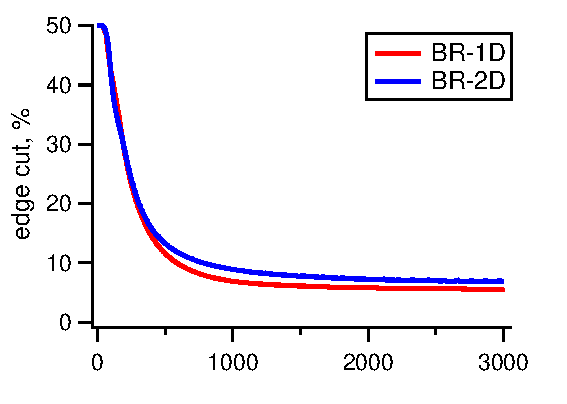
\includegraphics[width=0.99\textwidth]{pics/2da}
		\caption{bla.}
		\label{fig:2da}
	\end{minipage}
	\begin{minipage}[b]{0.33\textwidth}
		\centering
		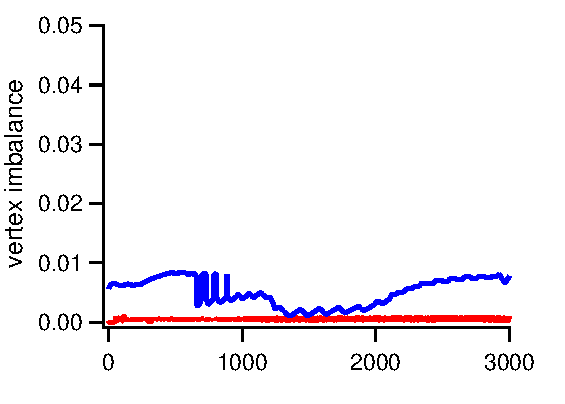
\includegraphics[width=0.99\textwidth]{pics/2db}
		\caption{bla.}
		\label{fig:2db}
	\end{minipage}
	\begin{minipage}[b]{0.33\textwidth}
		\centering
		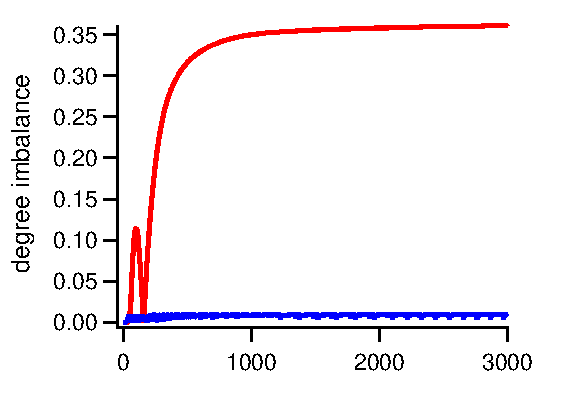
\includegraphics[width=0.99\textwidth]{pics/2dc}
		\caption{bla.}
		\label{fig:2dc}
	\end{minipage}
\end{figure}

%\subsection{Experiments with projections}
%\todo{Dmitry}

%First, we need to motivate the projection step. We will do it for $d=1$.
%\begin{itemize}
 % \item Consider LiveJournal graph. Compute $6$ plots: (i) quality vs iterations, (ii) number of moved vertices vs iterations, (iii) imbalance (max\_vertices/avg\_vertices) vs iterations. First do it for uniform projection ($3$ plots), then for binary-search-based one (another $3$ plots).
  
 % \item This one will motivcate the usage of approximate projection. Consider LiveJournal and build a plot "quality vs iterations" for $\eps=0$ (exact projection), $\eps=0.01$ ($1\%$ imbalance), $\eps=0.05$, and $\eps=0.1$.
%\end{itemize}
